% ltex: language=it
\chapter{Clustering}\label{chap:clustering} % (fold)
\section{Introduzione}\label{sec:introduzione} % (fold)
\begin{definition}{Clustering}{clustering}
    Con il termine \textbf{Clustering}, in italiano <<\red{raggruppamento}>>, si denota una famiglia di metodi \textit{non supervisionati} in grado di individuare \textbf{raggruppamenti intrinseci} (cluster) di pattern nello spazio multidimensionale, e opzionalmente di \red{definire in corrispondenza} di tali raggruppamenti le classi incognite.
    \\
    Il clustering ha applicazioni in numerose discipline (pattern recognition, machine learning, computer vision, data mining, data base) e pertanto ha sempre ricevuto un \textbf{notevole interesse}.
    \begin{center}
        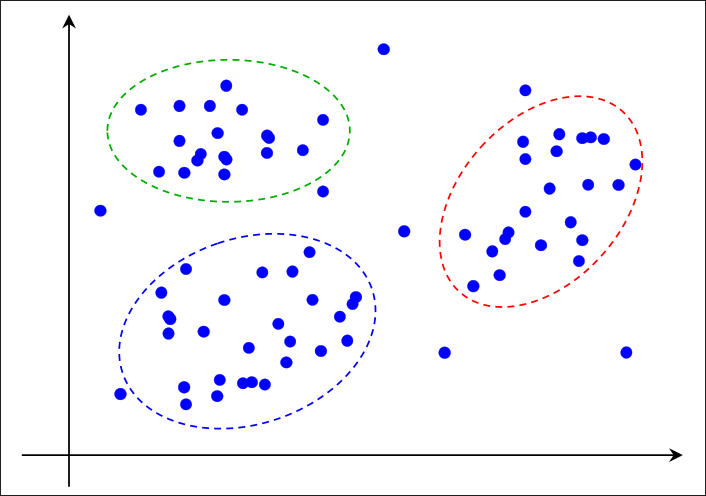
\includegraphics[width=.4\textwidth]{assets/clustering-def-visual.png}
    \end{center}
    Il problema è \textbf{molto complesso} (NP hard): determinare la soluzione ottima con ricerca esaustiva è possibile solo nei casi semplici (pochi pattern).
\end{definition}
\begin{lemma}{Quante soluzioni?}{}
    Dati $n$ pattern, assumendo di conoscere $s$, il numero di soluzioni è dell'ordine di $\dfrac{s^n}{s!}$ $\rightarrow$ approssimazione del numero di \textbf{Stirling} di seconda specie.
    \emptyln{}
    Se $s$ non è noto, il numero di soluzioni è dato dal numero di \textbf{Bell}, ottenibile sommando i casi precedenti per tutti i valori di $s$ da $1$ a $n$.
\end{lemma}
\begin{example}
    Nel caso $s = 2$ è molto semplice dimostrare che il numero di soluzioni è $2^{\dec n} - 1$: dati i $4$ pattern $\pg{A,\, B,\,C,\,D}$ e $s = 2$, le soluzioni di clustering sono $7$:
    \[
        \begin{matrix}
            \pt{A} \, \pt{B,C,D} \\
            \pt{B} \, \pt{A,C,D} \\
            \pt{C} \, \pt{A,B,D} \\
            \pt{D} \, \pt{A,B,C} \\
            \pt{A,B} \, \pt{C,D} \\
            \pt{A,C} \, \pt{B,D} \\
            \pt{A,D} \, \pt{B,C} \\
        \end{matrix}
    \]

\end{example}
%
\subsection{Criteri di Clustering}\label{sub:criteri_di_clustering} % (fold)
\textbf{Criteri} e algoritmi di clustering sono due cose ben distinte: i \textbf{primi} descrivono cosa si vuol ottenere specificando il grado di ottimalità di ogni soluzione ammissibile; i \textbf{secondi}, dato un criterio di clustering, forniscono una procedura algoritmica per determinare soluzioni che lo ottimizzano.
\emptyln{}
La maggior parte dei criteri di clustering sono definiti sulla base delle due \red{osservazioni} seguenti:
\begin{enumerate}
    \item i pattern all'interno dello stesso cluster devono essere tra loro più simili rispetto a pattern appartenenti a cluster diversi;
    \item i cluster sono costituiti da \red{nuvole di punti} a densità relativamente elevata separate da zone dove la densità è più bassa;
\end{enumerate}
Tra i diversi \red{criteri} possibili:
\begin{itemize}
    \item \textbf{minimizzare distanze dai centroidi}: minimizza la somma dei \red{quadrati delle distanze} dei pattern $x$ dai centroidi delle classi.
        \[
            J_e = \sum_{\for[][][s]}\sum_{x \in C_i}{\nm{x - \bar{x_i}}^2}, \qquad \bar{x_i} = \frac{1}{n_i}\sum_{x \in C_i}{x}
        \]
        dove $C_i$ è l'$i$-esimop cluster, $n_i$ il numero di pattern che contiene e $\bar{x_i}$ il suo centroide (media).
        \\
        È un \red{buon criterio per cluster a simmetria radiale} (circolari), ma penalizza forme allungate e cluster innestati, come ad esempio un cluster a forma di anello con all'interno un altro cluster.
    \item \textbf{minimizzazione distanze intra-classe}:
        \[
            J_e = \sum_{\for[][][s]}{n_i\cdot \bar{s_i}}, \qquad \bar{s_i} = \frac{1}{n_i}\sum_{x \in C_i}{f_s\pt{x,\,C_i}}
        \]
        dove $f_s\pt{x,\,C_i}$ è una misura di distanza tra $x$ e il cluster cui apparitene.
        Ad esempio:
        \begin{enumerate}[ref=\textbf{(\arabic*)}]
            \item \label{itm:dst_first} $f_s\pt{x,\,C_i} = \dfrac{1}{n_i}\displaystyle\sum_{x'\in C_i}{\nm{x- x'}^2}$\\
                criterio simile alla minimizzazione delle distanze dai centroidi;
            \item \label{itm:dst_second} $f_s\pt{x,\,C_i} = \displaystyle\min_{\substack{x'\in C_i \\ x' \ne x}}{\nm{x-x'}^2}$\\
                \red{non penalizza cluster allungati}, infatti affinché $f_s\pt{x,\,C_i}$ assuma valore ridotto, non è necessario che tutti i pattern di $C_i$ siano vicini a $x$, ma è sufficiente un vicino.
                Nell'esempio sotto, per $s = 2$: \ref{itm:dst_first} favorirebbe l'aggregazione, mentre la \ref{itm:dst_first} come da colori.
        \end{enumerate}
\end{itemize}
% subsection Criteri di Clustering (end)
% section Introduzione (end)
\section{Clustering Gerarchico}\label{sec:clustering_gerarchico} % (fold)

%
% section Clustering Gerarchico (end)
\section{Centroid-based Clustering}\label{sec:centroid_based_clustering} % (fold)

% section Centroid-based Clustering (end)
% chapter Clustering (end)
